\chapter{LITERATURE STUDY}
\label{chap:literaturestudy}

% Ubah bagian-bagian berikut dengan isi dari tinjauan pustaka

This chapter will explain the supporting theories that are used as references for this study.
The theories described in this chapter will be presented in a systematic order, starting from the most basic
to deeper explanations.

\section{Pose Estimation}
\label{sec:poseestimation}

% Contoh input gambar
\begin{figure}[ht]
  \centering

  % Ubah dengan nama file gambar dan ukuran yang akan digunakan
  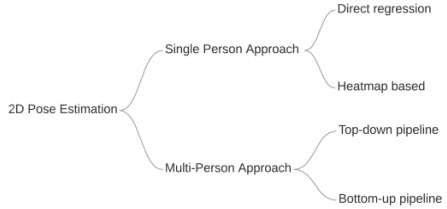
\includegraphics[scale=1]{gambar/taxonomy-pose-estimation.png}

  % Ubah dengan keterangan gambar yang diinginkan
  \caption{Taxonomy of pose estimation approaches}
  \label{fig:pose-estimation}
\end{figure}

Pose estimation is a heavily explored area with applications in gaming, animation, action recognition, activity tracking, and augmented reality.
In order to improve pose estimate outcomes, various approaches have been developed. These methods may generally be split into: Single-person and Multi-person approaches, 
as depicted in figure \ref{fig:pose-estimation}. The single-person approach is fundamentally a regression issue because it just determines the pose of a single person in an image, 
the person's position and an implicit number of keypoints are already known. However, the multi-person approach tries to solve an unconstrained problem because we do not know 
the positions and number of persons within the image \parencite{romeo}.

The single-person approach is divided into two frameworks based on the keypoint prediction method: directly regressing keypoints from the features (i.e. direct regression based framework)
or by generating heatmaps and inferencing keypoints via heatmap (i.e. heatmap based framework) \parencite{romeo}.
A direct regression-based framework can be implemented in various ways: as done by \parencite{toshev2014}, 
they presented DeepPose where their model uses a simple architecture with a convolutional layer, followed by a dense layer that will produce keypoint values in \emph{(x,y)}.
Other authors \parencite{carreira2015} suggested a technique that iteratively improves model output by feeding back mistake predictions, leading to a notable improvement in accuracy.

Then for a heatmap based framework, an alternative method can be used to generate heatmaps of all keypoints in the image
rather than directly predicting them. The final stick figure is then created using additional techniques to know the connection between keypoints or joints.
In \parencite{chen2014}, authors proposed a graphical model with pairwise
relations to make adaptive use of local image measurements. Later on, both the detection of joints and the prediction of their relationships can be accomplished using those local image measurements.
\parencite{newell2016} designed a \emph{"stacked hourglass"} network, that is closely similar to encoder-decoder architecture and is based on the sequential phases of pooling and upsampling.
They demonstrated the importance of repeated bottom-up, top-down processing with intermediate supervision for enhancing the effectiveness of human pose detection.

The multi-person approach is a more complex task because
the positions and number of persons within the image are unknown, therefore the framework has to detect keypoints and assemble an unknown number of persons. To overcome this task,
two pipelines have been proposed: top-down pipeline and bottom-up pipeline \parencite{romeo}.
Beginning with the detection of every person present in an image, the top-down pipeline creates bounding boxes. The following action uses each of the identified bounding boxes and applies a single-person method. 
For each person that is discovered, the single-person technique will generate keypoints, and then, as shown in Figure \ref{fig:top-down-approach}, the pipeline may include extra steps of post-processing and improving final results.

\begin{figure}[ht]
  \centering
  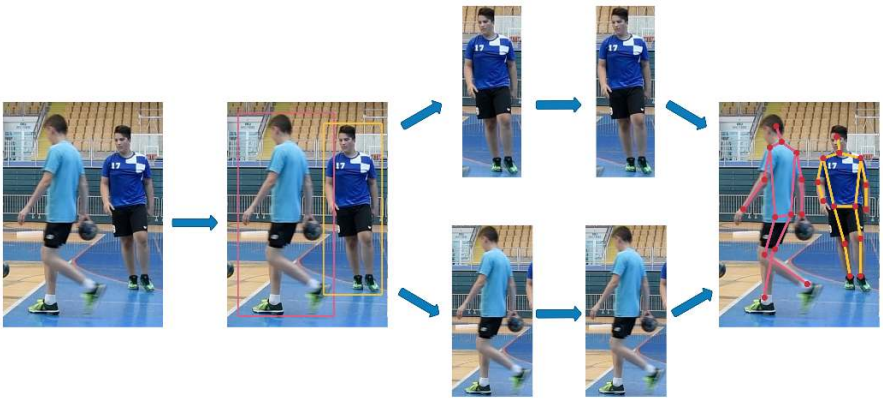
\includegraphics[scale=0.8]{gambar/top-down-approach.png}
  \caption{The top-down pipeline in multi-person approach for pose estimation}
  \label{fig:top-down-approach}
\end{figure}

Compare to a top-down pipeline, the bottom-up pipeline operates in reverse. The bottom-up pipeline begins by finding all of the keypoints, which are then connected to human instances, as seen in Figure \ref{fig:bottom-up-approach}. 
The bottom-up pipeline is probably quicker than the top-down pipeline because it doesn't detect human bounding boxes and runs pose estimation for each person individually.

\begin{figure}[ht]
  \centering
  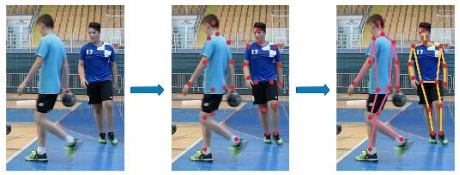
\includegraphics[scale=1.2]{gambar/bottom-up-approach.png}
  \caption{The bottom-up pipeline in multi-person approach for pose estimation.}
  \label{fig:bottom-up-approach}
\end{figure}

\section{Human Pose Estimation}
\label{sec:humanposeestimation}

Estimating human poses is one of the most challenging things in computer vision, which aims to determine the position or spatial location of certain points of a person's body (body parts/joints) from a given image or video.
Essentially it is a way to capture a set of coordinates by defining the human body joints like wrist, shoulder, knees, eyes, ears, ankles, and arms, which is a key point in images and videos that can describe a pose of a person. Then, when an image or video is given to the pose estimator model as input, it identifies the coordinates of these detected body parts and joints as output and a confidence score showing the precision of the estimations.
For many years, the main topic of discussion for numerous classical object detection applications has been the detection of persons.
With recent developments in machine-learning algorithms, computers can now understand human body language by performing pose detection and pose tracking. It has now reached a point where the hardware requirements to operate and the detection accuracy make them commercially viable.
Several industries, including security, business intelligence, health and safety, and entertainment, will be profoundly impacted by human pose estimate. Autonomous driving is one such application where this method has already shown its viability. Computers can sense and predict pedestrian behavior far more comprehensively with the use of real-time human pose detection and tracking, allowing for more consistent driving.

Pose estimation on humans can be divided into two techniques: 2D Pose Estimation and 3D Pose Estimation.
2D pose estimation is a type of pose estimation that can estimate the locations of the body joints in 2D space relative to input data (i.e., image or video frame). The location is represented with X and Y coordinates for each key point. On the other hand, 3D pose estimation transforms a 2D image into a 3D object by estimating an additional Z-dimension to the prediction. 3D pose estimation enables us to predict the accurate spatial positioning of a represented person or thing.

In the early days, the pose estimation job was treated as a part-based inference task, and there were two general groups of models. The first one is called appearance models, where features of body parts are first extracted by feature descriptors like Histogram of Oriented Gradient then distinct body parts are combined together.
Another group of models is deformable models or structural models. 
The performance of estimation models rapidly increases after deep convolutional networks are used for pose estimation. Researchers initially concentrate primarily on a well-cropped single-person posture estimate problem, which is a simplified sub-task. These days, more difficult situations, including pose estimation in a crowd, have become hot subjects thanks to the success of the more general multi-person pose estimation \parencite{song2021}.

\section{Humanoid Robot Pose Estimation}
\label{sec:humanoidrobotposeestimation}

Humanoid robots and people have similar shapes, which has both advantages and disadvantages. On the one hand, this allows us to start with approaches already in use for people, but on the other, it makes it harder for us to distinguish between people and humanoid robots \parencite{amini2021}.
as explained in Section \ref{sec:poseestimation}, in general, the effort to tackle the problem of pose estimation is vary depend on the number of persons (single-person or multi-person), for multiple persons can be categorized as a top-down or bottom-up approach.
In the top-down approach, the initial stage is to identify specific individuals, and the subsequent step is to implement pose estimation. The fact that the model's performance is closely associated with the performance of the person detector is one of the drawbacks of this approach. Although the state-of-the-art (SOTA) results are derived from this type of approach,  the runtime of such approaches is negatively affected by the number of persons present,
as a single-person pose estimator is run for each detection. Since the computational cost grows linearly as the number of users increases, performance is frequently not real-time \parencite{amini2021}.

Bottom-up techniques, on the other hand, are less reliant on the number of people in the image because they simultaneously identify body joints and classify them into individuals. Accurately grouping the detected keypoints in real-time is one of the bottom-up method's fundamental issues.
Recent methods arrange the identified keypoints into distinct instances using a greedy algorithm. In addition, compared to the top-down method, the bottom-up method's effectiveness is more influenced by the various scales of the people in a given image. Previous research has relied on high-resolution input size \parencite{papandreou2018} or the scale search method \parencite{cao2019} to address this issue. However, the inference time is growing as a result of these strategies.
A time-efficient method predicting keypoints at higher resolution was introduced by Cheng et al. \parencite{cheng2020}, narrowing the performance gap between bottom-up and top-down models.

There are three Pose Estimation Models for humanoid robots that we retrained with the
new dataset. All of them used bottom-up approaches. For a detailed explanation of each model is located in the next section.

\subsection{NimbRo's Model}
\label{subsec:nimbromodel}

NimbRo's model chose to use a similar architecture with NimbRo-Net and NimbRo-Net2 because it had such positive outcomes. Their model is an single-stage encoder-decoder network which takes an RGB image of
size \emph{w x h}. The model predicts heatmaps of both keypoints and limbs for scale 1/4 and only
heatmaps of keypoints for scale 1/2, where each scale is supervised with an intermediate loss \parencite{amini2021}. The full network architecture is depicted in Figure \ref{fig:nimbro-model-architecture}.

\begin{figure}[ht]
  \centering
  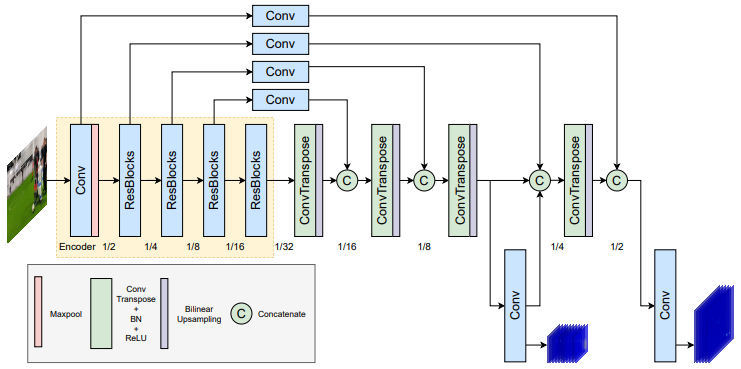
\includegraphics[scale=0.9]{gambar/nimbro-architecture.png}
  \caption{NimbRo's model architecture}
  \label{fig:nimbro-model-architecture}
\end{figure}

\subsection{YOLO-pose}
\label{subsec:yolopose}

Although this architecture is intended for humans, but it may be used for humanoid robot too, as explained in Section \ref{sec:humanoidrobotposeestimation}.
YOLO-pose is a single-shot approach like other bottom-up approaches. However, it doesn't use heatmaps. Rather, it associates all keypoints of a person with anchors. It is
based on YOLOv5 object detection framework and can be extended to other frameworks as well. Figure \ref{fig:YOLO-pose-architecture} illustrates the overall architecture with keypoint
heads for pose estimation. The Input image is passed through darknetcsp backbone that generates feature maps at
various scales {P3, P4, P5, P6}. PAnet is used for fusing these feature maps across multiple scales and the output is fed to detection
heads. Finally each detection head branches into box head and keypoint head \parencite{maji2022yolopose}.

\begin{figure}[ht]
  \centering
  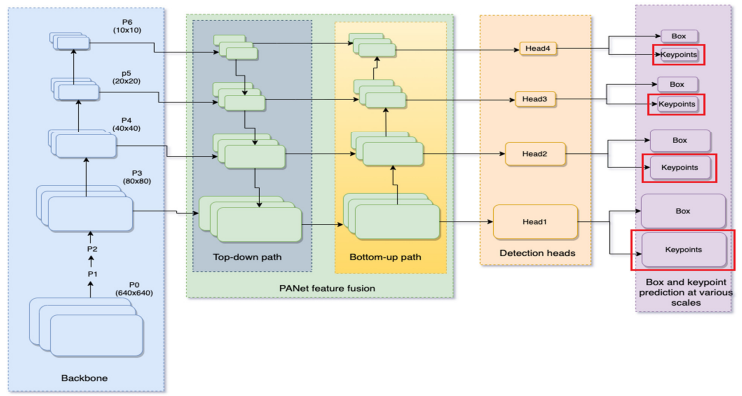
\includegraphics[scale=1]{gambar/yolo-architecture.png}
  \caption{YOLO-pose architecture.}
  \label{fig:YOLO-pose-architecture}
\end{figure}

\subsection{RCNN}
\label{subsec:rcnn}